\documentclass[12pt,a4paper]{article}
\usepackage[a4paper,top=1.5cm, bottom=1.5cm, left=1.5cm, right=1.5cm]{geometry}
\usepackage[T2A]{fontenc}
\usepackage[utf8]{inputenc}
\usepackage[russian]{babel}
\usepackage{amsmath}
\usepackage{amssymb}
\usepackage{graphicx}
\usepackage{floatrow}
\usepackage{booktabs}
\usepackage{wrapfig}
\usepackage{indentfirst}
\usepackage{lipsum}
\usepackage{subcaption}
\usepackage{float}
\usepackage{enumitem}
\restylefloat{table}

\newcommand{\figref}[1]{(см. рис. \ref{#1})}
\newcommand{\e}[1]{\text{$\cdot10^{#1}$}}

\title{Лабораторная работа 5.1.2 \\ Эффект Комптона}
\author{Симанкович Александр $\quad$ Паниман Александр\\ Б01-108}
\date{04.09.2023}

\begin{document}
	\maketitle
	
	\section*{Аннотация}
	
	В работе экспериментально подтверждена гипотеза об отрицательном сдвиге частоты при рассеянии $\gamma$-кванта на мишени (эффект Комптона). Косвенно определена энергия покоя электрона $mc^2 = (548 \pm ..)$ кэВ.
			
	\section*{Теоретическое введение}
	
	\subsection*{Модели комптоновского и рэлеевского рассеяний}
	При изучении рассеянного $\gamma$-излучения в его составе кроме основной частоты $\omega_0$ можно обнаружить излучение со смещенной ($\textit{уменьшенной}$) частотой. Данный эффект называется эффектом Комптона.
	
	Его обоснование можно дать, считая $\gamma$-излучение потоком квантов.

	\begin{figure}[h]
		\includegraphics[scale=0.65]{res/impulse_diagram.png}
		\caption{Векторная диаграмма рассеяния $\gamma$-кванта на электроне}
		\label{fig:impulse_diagram}
	\end{figure}
	
	Рассмотрим модель комптоновского рассеяния -- упругого соударения фотона и свободного электрона. Пользуясь векторной диаграммой и считая электрон покоящимся ($E_0 = mc^2$) получим следующие соотношения:
	$$ mc^2  + \hbar \omega_0 = \alpha m c^2 + \hbar \omega_1, $$
	$$ \frac{\hbar \omega_0}{c} = \alpha m v \cos \varphi + \frac{\hbar \omega_1}{c} \cos \theta, $$
	$$ \alpha m v \sin \varphi = \frac{\hbar \omega_1}{c} \sin \theta.$$
	
	Из данной системы получаем выражение для смещения длины волны:
	\begin{equation}
		\Delta \lambda = \lambda_0 - \lambda_1 = \Lambda_K (1 - \cos \theta),
		\label{eq:shift_lambda}
	\end{equation}
	где $\lambda_0$ -- начальная длина волны, $\lambda_1$ -- смещенная длина волны,
	$$ \quad \Lambda_K = \frac{h}{mc} = 2.42 \text{ пкм}, $$
	\textit{комптоновская длина волны электрона}.
	
	Обратим внимание, что смещение не зависит от вещества рассеивателя и энергии рассеиваемого кванта. Условием применимости данной модели является $E \gg E_{\text{связи}}$, где $E$ -- энергия фотонов, $E_{\text{связи}} \approx (0.1 \div 10) \text{ кэВ}$ -- энергия связи электрона в атоме.
	
	При рассеянии на связанном электроне имеет место классическое рэлеевское рассеяние. Оно описывается моделью упругого рассеяния на всем атоме. Условие применимости: $E_{\text{связи}} \gg E$.
	
	\subsection*{Влияние вещества рассеивателя и энергии фотонов}
	
	\begin{wrapfigure}{r}{7.0cm}
		\caption{Сечение взаимодействия фотонов с углеродом; \\
				 $\sigma_{\text{ф}}$ -- сечение фотоэффекта, \\
				 $\sigma_{\text{р}}$ -- сечение рэлеевского рассеяния, \\
				 $\sigma_{\text{к}}$ -- сечение комптоновского рассеяния, \\
				 $\sigma_{\text{tot}}$ -- общее сечение взаимодействия.
				 }
		\label{fig:cross_section}
		\includegraphics[width=5.5cm]{res/cross_section.png}
		\vspace{-10pt}
	\end{wrapfigure} 
	
	Сечения рассеяния зависят от атомного номера $Z$. Сечение рэлеевского рассеяния растет как $\sigma_{\text{р}} \sim Z^2$, поскольку электроны под действием фотона колеблются синфазно, складываются их амплитуды. В случае комптоновского электроны свободны и независимы, складываются интенсивности, поэтому $\sigma_{\text{к}} \sim Z$.
	
	Также сечения рассеяния зависят от энергии фотонов. На рис. $\ref{fig:cross_section}$ изображена данная зависимость. Обратим внимание, что существует зона ($\sim 20 \text{ кэВ}$), где комптоновское и рэлеевское рассеяния имеют одинаковые сечения. В этой зоне Комптон наблюдал одновременно две компоненты: исходную и смещенную.
	В нашем эксперименте фотоны обладают энергией $\sim 600 \text{ кэВ}$, поэтому мы увидим только смещенную компоненту.

	Кванты, попавшие в вещество, могут быть поглощены. Для этого существует два механизма: образование электрон-позитронных пар ($600 \text{ кэВ} < E_{\text{пор}} = 2mc^2 = 1.02 \text{ МэВ}$) и фотоэффект. При фотоэффекте из атома выбивается электрон, который далее теряет энергию на возбуждение других атомов. Энергия возбуждения излучается в виде мягких фотонов. 
	
	Таким образом, при исследовании высокоэнергетических рассеяных фотонов мы изучаем комптоновское рассеяние.

	\vspace{20pt}
	\section*{Методика эксперимента}
	
	
	\begin{figure}[H]
		\centering
		\begin{minipage}{0.6\textwidth}
			\centering
			\includegraphics[width=1.0\linewidth]{res/scheme.png}
			\label{fig:scheme}
		\end{minipage}%
		\begin{minipage}{0.4\textwidth}
			\centering
			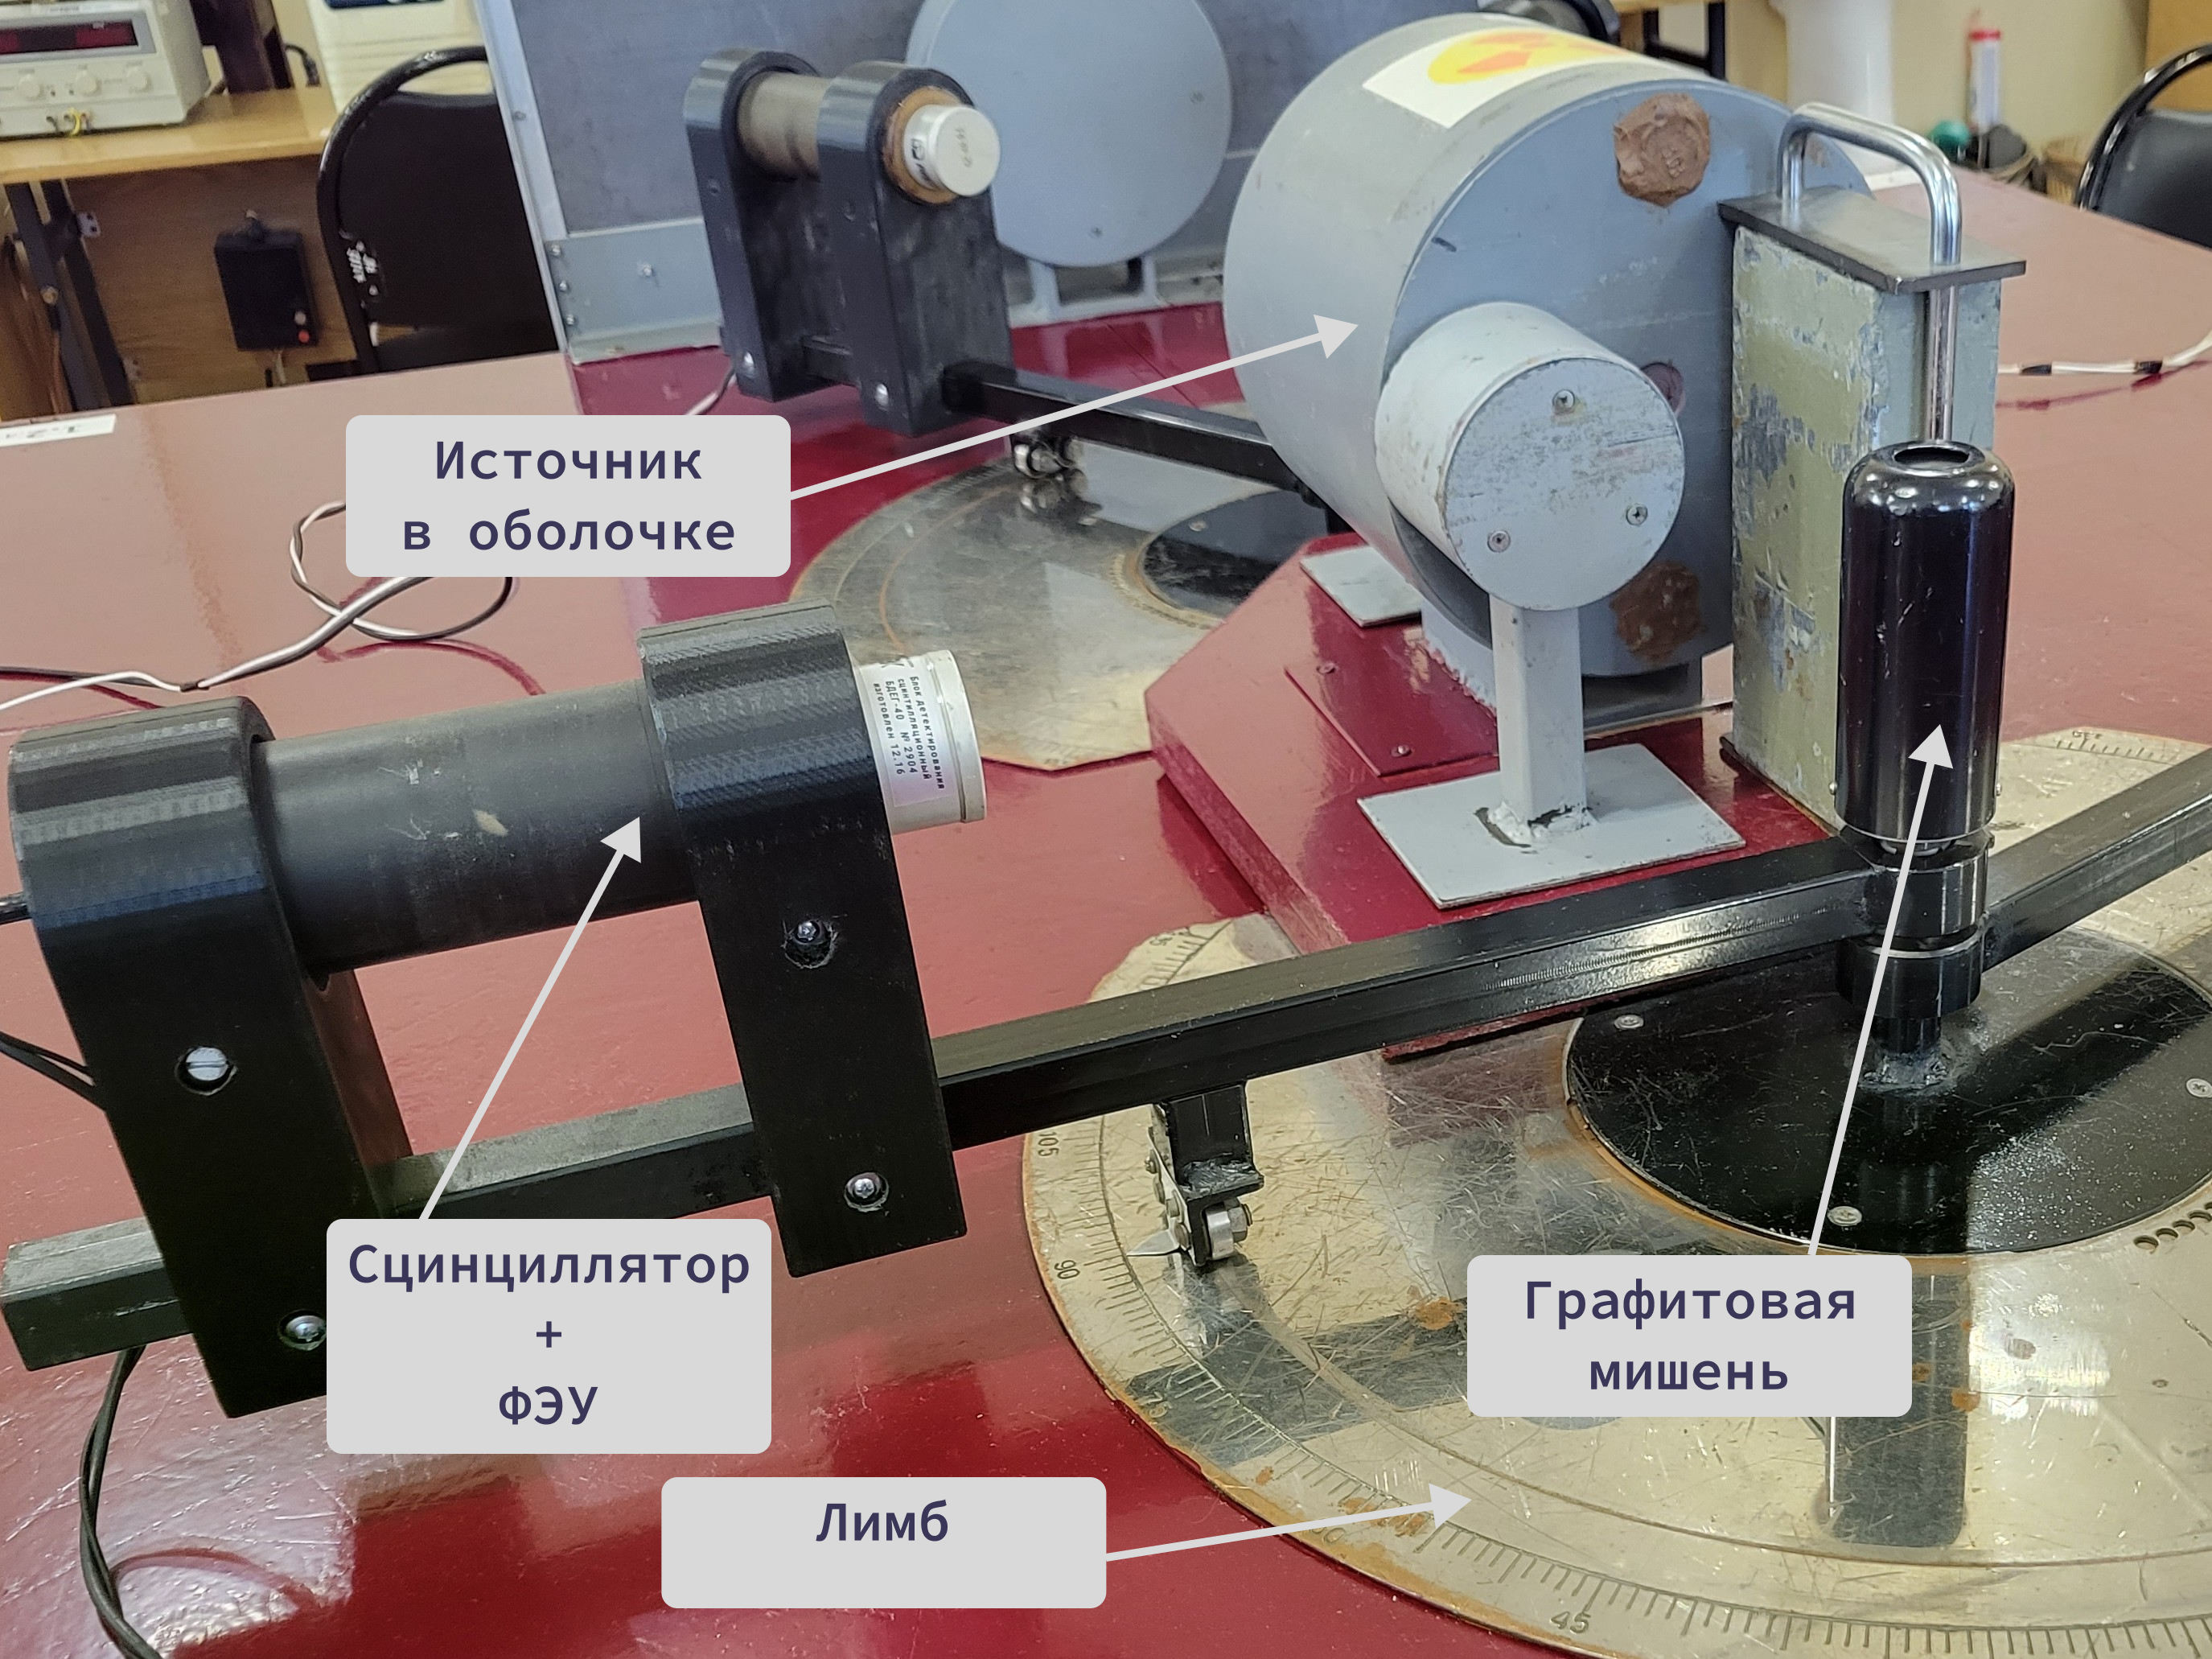
\includegraphics[width=1.0\linewidth]{photos/main.png}			\label{fig:main_photo}
		\end{minipage}
		\caption{Схема установки для изучения рассеяния $\gamma$-квантов}
	\end{figure}
		
	В качестве источника $\gamma$-квантов используется $^{137}$Cs с энергией квантов $E = 662$ кэВ, помещенный в свинцовый контейнер с коллиматором. Излучение попадает на графитовую мишень, в которой происходит рассеяние. Рассеянное излучение улавливается сцинтилляционным детектором NaI(Tl) в паре с фотоэлектронным умножителем (ФЭУ). Сигнал ФЭУ подается на ЭВМ с АЦП. ЭВМ получает спектр сигнала.
	
	\begin{figure}[H]
		\centering
		\begin{minipage}{0.5\textwidth}
			\centering
			\includegraphics[width=0.9\linewidth]{res/spectrum.png}
		\end{minipage}%
		\begin{minipage}{0.5\textwidth}
			\centering
			\includegraphics[width=0.9\linewidth]{photos/spectrum.jpg}
		\end{minipage}
		\caption{Спектр, получаемый на ЭВМ}
		\label{fig:spectrum}
	\end{figure}
	
	Рассеянный $\gamma$-квант порождает быстрые электроны в сцинтилляторе механизмами комптоновского рассеяния и фотоэффекта. Эти электроны возбуждают атомы в стинцилляторе. Возбужденные атомы излучают фотоны оптического диапазона, которые улавливаются ФЭУ.
	При комптоновском рассеянии $\gamma$-квант передает лишь часть энергии и создает шумовую часть спектра. При фотоэффекте происходит \textit{полное поглощение} кванта электроном, в этом случае амплитуда вспышек пропорциональна полной энергии кванта. Положение этого пика однозначно определяет энергию $\gamma$-кванта.
	
	Для численной обработки перепишем формулу (\ref{eq:shift_lambda}):
	\begin{equation*}
		\frac{1}{\varepsilon(\theta)} - \frac{1}{\varepsilon_0} = 1 - \cos \theta,
		\label{eq:shift_epsilon}
	\end{equation*}
	где $\varepsilon(\theta)$ -- энергия рассеянных на угол $\theta$ квантов $\varepsilon_0$ -- энергия исходных квантов, выраженные в единицах $mc^2$ ($m$ -- масса электрона).
	
	Переписывая для каналов ЭВМ в спектре:
	\begin{equation}
		\frac{1}{N(\theta)} - \frac{1}{N_0} = A (1 - \cos \theta),
		\label{eq:shift_n}
	\end{equation}
	где соответствующие $N$ -- номера каналов, $A$ -- коэффициент пропорциональности: $\varepsilon = A N$.
	
	Также мы можем вычислить энергию покоя электронов, на которых происходит рассеяние:
	\begin{equation}
		mc^2 = E(0) \frac{E(90)}{E(0) - E(90)} = E_{\gamma} \frac{N(90)}{N(0) - N(90)},
	\end{equation}
	где $N(\theta)$ -- номер канала, на котором находится пик полного поглощения для угла $\theta$, $E_{\gamma} = 662$ кэВ -- начальная энергия квантов.

	\section*{Результаты}
		В соответствии с методикой, указанной выше, получаем спектры для углов в диапазоне $\theta = (0 \div 110)^{\circ}$. Исходя из формулы ($\ref{eq:shift_n}$) по положениям фотопика строим график $\frac{1}{N} = f(1 - \cos \theta)$.

		\begin{figure}[h]
			\centering
	        \includegraphics[width=0.8\textwidth]{res/graph.png}
	        \caption{Зависимость энергии рассеянного кванта от угла рассеяния}
		\end{figure}
		
        Аппроксимируя график прямой имеем: $k = 0.00130, \; b = 0.00107$.

        Из аппроксимации получаем: $N(0) = 931.42, \; N(90) = 421.73$.
        Откуда энергия покоя электрона: $mc^2 = (547.75 \pm ..)$ кэВ.

	\section*{Заключение и выводы}
	
	Данная работа подтверждает существование эффекта Комптона.
	
	Проверена корректность зависимости (\ref{eq:shift_lambda}). Получено значение энергии покоя электрона $mc^2 = (548 \pm ..)$ кэВ. Справочное значение: $mc^2 = 511$ кэВ.
	
	
	%Данная работа подтверждает существование эффекта Холла в полупроводниках.
	%
	%Получено значение коэффициента Холла $ R_H = (6.9 \pm 0.4) \cdot 10^{-4} \; \frac{\text{м}^3}{\text{Кл}} $. Также в работе оценено значение концентрации носителей тока в образце $ n = (8.7 \pm 0.4) \cdot 10^{21} \; \frac{1}{\text{м}^3} $, удельная проводимость $ \sigma_0 = (309 \pm 27) \; \frac{1}{\text{Ом} \cdot \text{м}} $, подвижность носителей $ b = \frac{\sigma_0}{e n} = (2230 \pm 220) \; \frac{\text{см}^2}{\text{В} \cdot \text{с}} $.
	%
	%Справочные данные для данного образца германия отсутствуют, большинство параметров зависят от степени легирования. Значения подвижности носителей зависит от легирующего элемента и лежат в пределах\footnote{Эффект Холла в германии, легированном разными примесями, Г. П. Гайдар, Е. Ю. Гайворонская, 2017} $(2000 \div 3000) \; \frac{\text{см}^2}{\text{В} \cdot \text{с}}$.
	%
	
	\newpage
	\section*{Приложение 1. Измерения}
	
	\begin{table}[h]
		\centering
		\begin{tabular}{rrrrrrl}
			$\theta, ^{\circ}$ & $N$ (фотопик) & Ширина cлева & Ширина cправа & Плато слева & Плато cправа & ?\\[0pt]
			\hline
			0 & 965 & 929 & 1002 & 957 & 975 & \\[0pt]
			7 & 892 & 847 & 935 & 885 & 899 & x\\[0pt]
			20 & 881 & 830 & 923 & 857 & 896 & \\[0pt]
			30 & 809 & 748 & 858 & 799 & 820 & \\[0pt]
			40 & 723 & 677 & 760 & 704 & 740 & \\[0pt]
			50 & 627 & 579 & 670 & 608 & 643 & \\[0pt]
			60 & 581 & 525 & 616 & 563 & 596 & \\[0pt]
			70 & 512 & 469 & 548 & 489 & 534 & \\[0pt]
			80 & 462 & 427 & 490 & 444 & 477 & \\[0pt]
			90 & 424 & 392 & 434 & 402 & 424 & \\[0pt]
			100 & 385 & 360 & 402 & 372 & 393 & \\[0pt]
			110 & 359 & 340 & 374 & 352 & 365 & \\[0pt]
			\hline
		\end{tabular}
		\label{tab:measurements}
		\caption{Положение фотопика от угла рассеяния}
		
	\end{table}
	
\end{document}
